\documentclass{beamer}
\usepackage[utf8]{inputenc}

\usetheme{Madrid}
\usecolortheme{default}
\usepackage{amsmath,amssymb,amsfonts,amsthm}
\usepackage{txfonts}
\usepackage{tkz-euclide}
\usepackage{listings}
\usepackage{adjustbox}
\usepackage{array}
\usepackage{tabularx}
\usepackage{gvv}
\usepackage{lmodern}
\usepackage{circuitikz}
\usepackage{tikz}
\usepackage{graphicx}

\setbeamertemplate{page number in head/foot}[totalframumber]

\usepackage{tcolorbox}
\tcbuselibrary{minted,breakable,xparse,skins}



\definecolor{bg}{gray}{0.95}
\DeclareTCBListing{mintedbox}{O{}m!O{}}{%
  breakable=true,
  listing engine=minted,
  listing only,
  minted language=#2,
  minted style=default,
  minted options={%
    linenos,
    gobble=0,
    breaklines=true,
    breakafter=,,
    fontsize=\small,
    numbersep=8pt,
    #1},
  boxsep=0pt,
  left skip=0pt,
  right skip=0pt,
  left=25pt,
  right=0pt,
  top=3pt,
  bottom=3pt,
  arc=5pt,
  leftrule=0pt,
  rightrule=0pt,
  bottomrule=2pt,
  toprule=2pt,
  colback=bg,
  colframe=orange!70,
  enhanced,
  overlay={%
    \begin{tcbclipinterior}
    \fill[orange!20!white] (frame.south west) rectangle ([xshift=20pt]frame.north west);
    \end{tcbclipinterior}},
  #3,
}
\lstset{
    language=C,
    basicstyle=\ttfamily\small,
    keywordstyle=\color{blue},
    stringstyle=\color{orange},
    commentstyle=\color{green!60!black},
    numbers=left,
    numberstyle=\tiny\color{gray},
    breaklines=true,
    showstringspaces=false,
}
%------------------------------------------------------------
%This block of code defines the information to appear in the
%Title page
\title %optional
{1.8.19}
\date{September 14,2025}
%\subtitle{A short story}

\author % (optional)
{EE25BTECH11002 - Achat Parth Kalpesh}



\begin{document}


\frame{\titlepage}

\begin{frame}{Question}
If $\vec{Q}$\brak{0, 1} is equidistant from $\vec{P}$\brak{5, -3} and $\vec{R}$\brak{x, 6}, find the values of x. Also find the distances $\vec{QR}$ and $\vec{PR}$.
\end{frame}



\begin{frame}{Theoretical Solution}

Let the vectors for the given points $\vec{P}$, $\vec{Q}$ and $\vec{R}$ be
\begin{align}
    \vec{P} = \myvec{5 \\ -3}, \quad \vec{Q} = \myvec{0 \\ 1}, \quad \vec{R} = \myvec{x \\ 6}
\end{align}
It is given that $\vec{Q}$ is equidistant from $\vec{P}$ and $\vec{R}$.
\begin{align}
\norm{\vec{P} - \vec{Q}} = \norm{\vec{R} - \vec{Q}}
\end{align}
Squaring both sides,
\begin{align}
\norm{\vec{P} - \vec{Q}}^2 = \norm{\vec{R} - \vec{Q}}^2
\end{align}
The squared norm of a vector $\vec{v}$ is given by $\vec{v}^\top\vec{v}$.
\begin{align}
\brak{\vec{P} - \vec{Q}}^\top \brak{\vec{P} - \vec{Q}} = \brak{\vec{R} - \vec{Q}}^\top \brak{\vec{R} - \vec{Q}}
\end{align}

\end{frame}

\begin{frame}{Theoretical Solution}
\begin{align}
\brak{\vec{P}^{\top} - \vec{Q}^{\top}} \brak{\vec{P} - \vec{Q}} &= \brak{\vec{R}^{\top} - \vec{Q}^{\top}} \brak{\vec{R} - \vec{Q}}\\
\vec{P}^{\top}\vec{P} - 2\vec{Q}^{\top}\vec{P} &= \vec{R}^{\top} \vec{R} - 2\vec{R}^{\top}\vec{Q}\\
\myvec{5 & -3}\myvec{5 \\ -3} - 2\myvec{0 & 1}\myvec{5 \\ -3} &= \myvec{x & 6}\myvec{x \\ 6} - 2\myvec{x & 6}\myvec{0 \\ 1}\\
25 + 9 + 6 &= x^2 + 36 -12 \\
x^2 &= 16 \\
    \implies x &= \pm 4
\end{align}

\end{frame}

\begin{frame}{Theoretical Solution}
Therefore, the two possible vectors for $\vec{R}$ are:
\begin{align}
\vec{R}_1 = \myvec{4 \\ 6}  \\  \vec{R}_2 = \myvec{-4 \\ 6}
\end{align}




\begin{align}
     \norm{\vec{Q} - \vec{R}}&= \norm{\vec{P} - \vec{Q}} = \sqrt{5^2 + \brak{-4}^2} = \sqrt{41} \approx 6.40
\end{align}
\end{frame}



\begin{frame}{Theoretical Solution}
\begin{itemize}
    \item For $\vec{R}_1 = \myvec{4 \\ 6}$:
    \begin{align}
     \norm{\vec{R_1} - \vec{P}} &= \norm{ \myvec{4 - 5 \\ 6 - \brak{-3}}}  = \norm{ \myvec{-1 \\ 9}} \\
    &= \sqrt{\brak{-1}^2 + 9^2} = \sqrt{82} \approx 9.06
    \end{align}
    \item For $\vec{R}_2 = \myvec{-4 \\ 6}$:
    \begin{align}
    \norm{\vec{R}_2 - \vec{P}} &= \norm{\myvec{-4 - 5 \\ 6 - (-3)}}  = \norm{\myvec{-9 \\ 9}} \\
    &= \sqrt{\brak{-9}^2 + 9^2} = \sqrt{162} = 9\sqrt{2} \approx 12.73
    \end{align}
\end{itemize}
\end{frame}

\begin{frame}[fragile]
    \frametitle{C code}
    \begin{lstlisting}
#include <stdio.h>
#include <math.h>
void formula(double *P, double *Q, double *R){
    double sum1 = 0, sum2 = 0;
    for (int i=0; i<2; i++) {
        sum1 += pow(P[i] - Q[i], 2);
        sum2 += pow(R[i] - Q[i], 2);
    }
    if (sum1 == sum2) {
        printf("Q is equidistant from P and R.");
    }
}
    \end{lstlisting}
\end{frame}

\begin{frame}[fragile]
    \frametitle{Python Code}
    \begin{lstlisting}
import numpy as np
import matplotlib.pyplot as plt
from numpy import linalg as LA
import ctypes
import os

# --- Part 1: Mathematical Solution ---
Q_coords = (0, 1)
P_coords = (5, -3)
# From calculation, x = 4 or x = -4
R1_coords = (4, 6)
R2_coords = (-4, 6)

# Calculate distances using numpy
P = np.array(P_coords)
Q = np.array(Q_coords)
R1 = np.array(R1_coords)
R2 = np.array(R2_coords)
    \end{lstlisting}
\end{frame}


\begin{frame}[fragile]
    \frametitle{Python Code}
    \begin{lstlisting}
dist_QR1 = LA.norm(R1 - Q)
dist_PR1 = LA.norm(R1 - P)
dist_PR2 = LA.norm(R2 - P)

print(f"Distance QR: {dist_QR1:.2f}")
print(f"Distance PR1 (for x=4): {dist_PR1:.2f}")
print(f"Distance PR2 (for x=-4): {dist_PR2:.2f}\n")

# --- Part 2: C Code Integration using ctypes ---
try:
    # Load the shared library
    geom_lib = ctypes.CDLL('./formula.so')

    # Define the function signature
    c_double_p = ctypes.POINTER(ctypes.c_double)
    geom_lib.formula.argtypes = [c_double_p, c_double_p, c_double_p]
    geom_lib.formula.restype = None
    \end{lstlisting}
\end{frame}


\begin{frame}[fragile]
    \frametitle{Python Code}
    \begin{lstlisting}
    # Prepare data for C function
    P_c = (ctypes.c_double * 2)(*P)
    Q_c = (ctypes.c_double * 2)(*Q)
    R1_c = (ctypes.c_double * 2)(*R1)
    R2_c = (ctypes.c_double * 2)(*R2)

    # Call the C function for both solutions
    print("Calling C function with R1(4, 6):")
    geom_lib.formula(P_c, Q_c, R1_c)
    print("\nCalling C function with R2(-4, 6):")
    geom_lib.formula(P_c, Q_c, R2_c)

except (OSError, AttributeError) as e:
    print(f"Error loading or using the C library: {e}")
    \end{lstlisting}
\end{frame}


\begin{frame}[fragile]
    \frametitle{Python Code}
    \begin{lstlisting}
# --- Part 3: Plotting ---
Q = Q.reshape(-1, 1)
P = P.reshape(-1, 1)
R1 = R1.reshape(-1, 1)
R2 = R2.reshape(-1, 1)

r = LA.norm(P - Q) # Radius is distance QP

# Helper function to generate circle points
def circ_gen(O, r):
    len = 100
    theta = np.linspace(0, 2*np.pi, len)
    x_circ = np.zeros((2, len))
    x_circ[0, :] = r * np.cos(theta)
    x_circ[1, :] = r * np.sin(theta)
    x_circ = (x_circ.T + O.T).T
    return x_circ
    \end{lstlisting}
\end{frame}

\begin{frame}[fragile]
    \frametitle{Python Code}
    \begin{lstlisting}
    x_circ = circ_gen(Q, r)
x_line = np.linspace(-10, 10, 100)
y_line = np.full_like(x_line, 6)

plt.figure(figsize=(8, 8))
plt.plot(x_circ[0, :], x_circ[1, :], label='Circle centered at Q')
plt.plot(x_line, y_line, label='Line y = 6')

# Plot lines connecting points
plt.plot([P[0,0], R1[0,0]], [P[1,0], R1[1,0]], 'g--', label='Line $PR_1$')
plt.plot([P[0,0], R2[0,0]], [P[1,0], R2[1,0]], 'm--', label='Line $PR_2$')
    \end{lstlisting}
\end{frame}

\begin{frame}[fragile]
    \frametitle{Python Code}
    \begin{lstlisting}
# Plot and label the points
points = np.hstack((P, Q, R1, R2))
plt.scatter(points[0, :], points[1, :], s=50, color='red', zorder=5)
point_labels = ['P(5,-3)', 'Q(0,1)', 'R1(4,6)', 'R2(-4,6)']

for label, (x, y) in zip(point_labels, points.T):
    plt.annotate(label, (x, y), textcoords="offset points", 
    xytext=(0,10), ha='center')

# Plot formatting
plt.xlabel("x-axis")
plt.ylabel("y-axis")
plt.title("Visual Representation of the Solution")
plt.legend()
plt.grid(True)
plt.axis('equal')
plt.show()
    \end{lstlisting}
\end{frame}

\begin{frame}{Python Plot}
    \begin{figure}
        \centering
        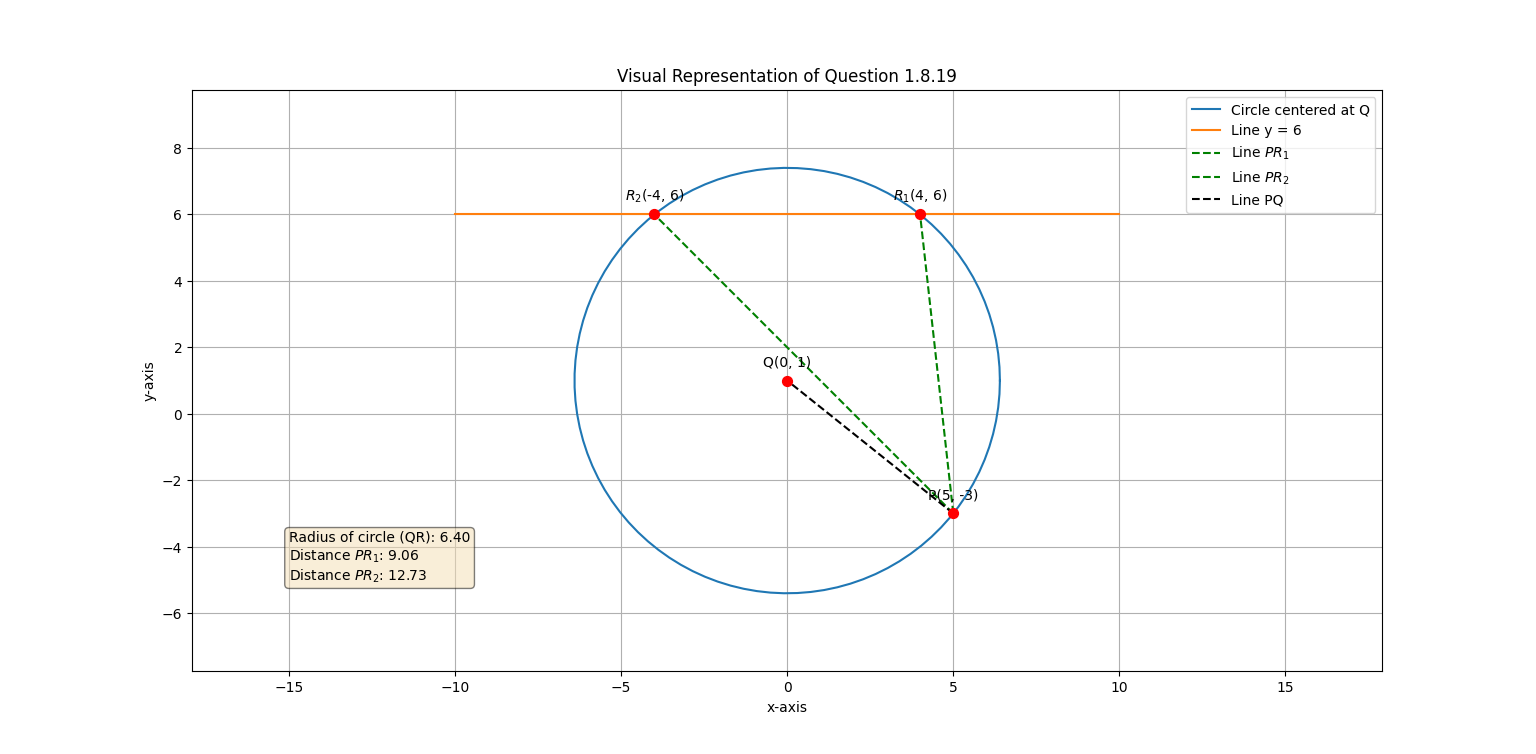
\includegraphics[width=0.8\columnwidth]{../figs/figure_c.png}
        \caption{Visual representation of the solution. The points $R_1$ and $R_2$ are the intersections of the circle centered at Q and the line $y=6$.}
        \label{fig:fig}
    \end{figure}
\end{frame}

\end{document}
